% REMEMBER: You must not plagiarise anything in your report. Be extremely careful.

\documentclass{l4proj}

    
%
% put any additional packages here
%
\usepackage{hyperref}
\hypersetup{
    colorlinks=true,
    linkcolor=black,    
    urlcolor=cyan,
    citecolor=black
}

\begin{document}

%==============================================================================
%% METADATA
\title{Espruino Tools - An asynchronous JavaScript library to control remote embedded devices [JavaScript, Promise, Arduino]}
\author{Callum McLuskey}
\date{24 March, 2023}


\maketitle

%==============================================================================
%% ABSTRACT
\begin{abstract}

    The personal usage of remote embedded devices is a growing area in engineering allowing for anybody to get started building robotics systems at home or even develop skill sets in programming and electronic engineering. A big name in this scene is Arduino a product which allows hobbyists to build and design systems to suit personal project needs; The Espruino project takes this in a different direction by utilising a JavaScript interpreter which aims to bring remote embedded systems programming to the web. This project intends to improve the development experience of remote embedded devices by refining the process and allowing users to focus more on their ideas and less on the semantics required to implement them. To achieve this the project introduces many packages providing functionality such as easy device connection[ADD LINK], peer-to-peer[ADD LINK] connection for mobile device inputs to be used, and the refined syntax to allow developers to get started regardless of skill or prior knowledge with wide and detailed documentation to avoid confusion when developing. In addition to this to further ease development, a CLI tool has been developed to create projects preset with all the functionality a beginner user could need, setting anybody up for programming Espruino devices, an activity which had no clear direction before of how to be done. By utilising user studies throughout the project a variety of users from different experience levels have been considered during the development process allowing for the project to be as accessible as possible.

\end{abstract}

\def\consentname {Callum McLuskey} % your full name
\def\consentdate {23 March 2023} % the date you agree

\educationalconsent

\tableofcontents
\listoffigures

%==============================================================================
%% Notes on formatting
%==============================================================================
% The first page, abstract and table of contents are numbered using Roman numerals and are not
% included in the page count. 
%
% From now on pages are numbered
% using Arabic numerals. Therefore, immediately after the first call to \chapter we need the call
% \pagenumbering{arabic} and this should be called once only in the document. 
%
% Do not alter the bibliography style.
%
% The first Chapter should then be on page 1. You are allowed 40 pages for a 40 credit project and 30 pages for a 
% 20 credit report. This includes everything numbered in Arabic numerals (excluding front matter) up
% to but excluding the appendices and bibliography.
%
% You must not alter text size (it is currently 10pt) or alter margins or spacing.
%
%
%==================================================================================================================================
%
% IMPORTANT
% The chapter headings here are **suggestions**. You don't have to follow this model if
% it doesn't fit your project. Every project should have an introduction and conclusion,
% however. 
%
%==================================================================================================================================
\chapter{Introduction}

% reset page numbering. Don't remove this!
\pagenumbering{arabic} 


\section{Motivation}

\text 
The area of remote embedded systems has seen significant growth in recent years due to the growing need for interconnected devices and the Internet of Things (IoT). It offers developers the chance to craft physical objects that interact with the real world, resulting in a final product they can take pride in. However, the current setup of remote embedded systems, like Arduino, has a challenging learning curve due to the utilization of C++ as the programming language alongside a requirement for developers to install drivers to get started.
\\ \\
An alternate solution to this is presented by Espruino devices, which make use of JavaScript, a language that is more accessible to a broader range of developers. The usage of JavaScript promotes learning a language which has a wide variety of use cases such as web development, machine learning and even mobile apps. Espruino presents a reduced entry barrier and eliminates the requirement to learn a less than beginner friendly low level language such as C/C++, which can be daunting for some and for most will not translate to other aspects of their coding career. This makes it easier for developers to commence with remote embedded systems and begin constructing their projects.
\\ \\
Even though using Espruino devices can tackle some of the issues linked to traditional remote embedded systems, it still gives a restricted comprehension of JavaScript and its fundamental technologies as developers are not getting exposed to aspects of the language outside of the native language. This can result in a limited skill set that is not readily transferable to other areas of software engineering.
\\ \\
This project aims to tackle these challenges by providing developers with a modern JavaScript-based platform for building their remote embedded systems. By utilizing contemporary JavaScript, developers will gain a deeper understanding of the language and its features, as well as acquire in-demand skills that can be applied to other areas of software engineering.
\\ \\
This project aims to help prepare future programmers and software engineers for work within the embedded systems allowing them to achieve working systems as well as allowing for the development of in-demand skills through the usage of modern JavaScript with easy access to work with any modern JavaScript of their choice. By incorporating embedded device development into the learning process beginner programmers are able to engage with tangible creations whilst introducing them into the idea of bringing in other sectors of industry into their programming.

\section{Aims}

\text This effort will create a collection of packages aimed at lowering the threshold for individuals looking to get into programming in the remote embedded systems area, yet still offering benefits for experienced coders through its streamlining of the current Espruino implementation. Additionally, these modules are constructed with a strong emphasis on web technologies, providing both novice and seasoned developers with an opportunity to deepen their understanding of current web technologies while working on their embedded systems.
\subsection{Goals}
\text From the aims stated above the problem is broken down into the following focal points.
\\
\subsubsection{Beginner friendly platform} \hfill\\
\text Provide a platform for beginner programmers to easily get started with embedded systems programming without advanced programmers being deterred.
\\
\subsubsection{Easy browser to device communication} \hfill\\
\text Introduce the idea of browser to device communication enabling programmers to have further control over input to devices by allowing them to utilise devices such as mobile phones, laptops or tablets as means to control their devices even using the device as a compliment to the web applications.
\\
\subsubsection{Reduce development time} \hfill\\
\text Allow developers to focus more on their ideas and less on the semantics of implementing them or navigating bad documentation or cryptic method naming schemes by following industry standard conventions and language specific rules alongside an in-depth and well populated documentation site.
\\
\subsubsection{Bring everything into one place} \hfill\\
\text Remove the requirement for developers to worry about compatibility with third party dependencies by providing a feature rich ecosystem with easy extension for more experienced developers.
\\
\subsubsection{Easy creation sharing}\hfill\\
\text Provide a service which allows developers to easily show off their creations; allow users to host their projects without cost, hassle or knowledge in web servers.
\\
\subsubsection{Flexibility in development style}\hfill\\
\text Build an ecosystem which works regardless of how the developer decides to work by supporting package importing through all available avenues as well as documentation/demos which show off this functionality to allow for no confusion in the process.
\\


%==================================================================================================================================
\chapter{Background}

\section{The Current state of learning programming}

Learning how to program is an increasingly popular avenue for young professionals in recent years due to the market demand for software engineers and appeal of working in a creative, challenging and constantly evolving field; because of this increase in desire to learn how to code many people are funneled into the following avenues each with their own advantages and drawbacks.

\subsection{Formal Teaching of programming}
Many students find themselves learning how to program for the first time during a degree at university. Within the University of Glasgow the current method of teaching provides students with an intricate understanding of programming without a proper understanding of how programming results in an end software product. This approach to programming is aimed towards providing students with enough knowledge to understand the following course content such as algorithms and data structures.
\begin{itemize}
    \item Maybe a quick survey surrounding if students know how to turn their programming language knowledge into working products or how learning for example python relates to something like a web application.
\end{itemize}


\subsection{Code boot camps / online courses}
On the other side of the spectrum many aspiring software engineers take the route of code "boot camps" such as \href{https://www.freecodecamp.org/}{freeCodeCamp} or \href{https://www.schoolofcode.co.uk/}{School of Code}. These intensive courses have the goal of producing work ready skills whilst avoiding theoretical skills that help programmers gather a better understanding of how the underlying programs work. These courses are usually highly specialised and web focuses meaning developers can potentially finish with a lack of transferable skills harming the ability for developers to transfer to new technologies and grow as a developer. An issue that comes with code boot camps are programmers who have followed tutorials word for word without absorbing the content itself resulting in people who believe they know how to develop systems without any real idea.

\subsection{The job market}
The job market for software engineers is an ever evolving market which rewards a developers skill to constantly learn on the job. Despite this languages such as JavaScript remain within the most used within the area within the \href{https://survey.stackoverflow.co/2022/#technology-most-popular-technologies}{Stack Overflow Developer Survey} we can see current trends. With an ever evolving job market it is important that anybody learning to program is able to understand the fundamentals of systems through the construction of systems whilst also understanding why these systems work at the lower level.

\section{Espruino Devices}
\text 
The \href{https://www.espruino.com/}{Espruino micro-controller} provides an innovative solution for individuals seeking to materialise their electronics project aspirations. With a JavaScript interpreter and in-built amenities such as WiFi and Bluetooth, this device makes it effortless for individuals of diverse programming proficiency to dive in. The Espruino ecosystem caters to hobbyists and students eager to learn about electronics and programming. These micro-controllers can be blended seamlessly with other hardware and software systems, opening up a world of possibilities for electronics projects.

    
\subsection{UART}
\text Espruino devices communicate with the browser by utilising the UART protocol, or Universal Asynchronous Receiver/Transmitter, a widely used communication protocol in the world of micro-controllers and embedded systems. It doesn't require a fixed clock rate between the sender and receiver and instead uses start and stop bits for data transmission synchronization. UART works by utilising a transmission control line (TX) and a reception control line (RX); UART will begin by sending a start bit from TX to RX to initiate the start of a data transfer from here data is transferred bit by bit over a single data line starting with the least significant bit (LSB) and finishing with the most significant bit (MSB) following this a stop bit is sent to signal data transfer has finished. This is detailed in figure \ref{fig:UART}.

\begin{figure}[!ht]
\begin{center}
    % ADD FIGURE DETAILS LIKE A CAPTION
    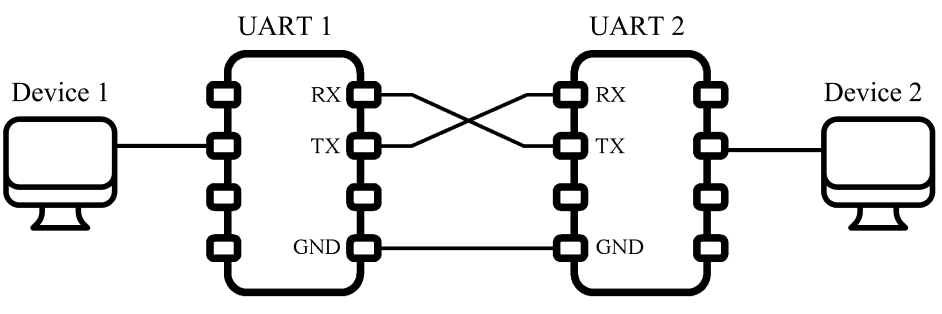
\includegraphics[width=60mm,scale=0.5]{dissertation/images/UART_diagram.png}
\end{center}
\caption{UART}
    \label{fig:UART}
\end{figure}

\subsection{WebBluetooth}
\text UART connection with a web browser as mentioned above is facilitated via \href{https://developer.mozilla.org/en-US/docs/Web/API/Web_Bluetooth_API}{WebBluetooth}. WebBluetooth is an aspect of the Web API that facilitates communication between web applications and Bluetooth Low Energy (BLE) devices. This technology allows web developers to control and access BLE devices using JavaScript, providing a streamlined and standardized approach.

WebBluetooth represents a milestone in the integration of BLE devices into the web, as it offers a common platform for web developers to interact with these devices, regardless of their origin or operating system. It expands the possibilities for BLE devices, including the ability to control smart home technology or track fitness information through a web application.

\section{Package Development}

Software packages are method of extending the functionality of a given language through externally written code. With the wide adoption of node.js in web development many package developers have adopted the UNIX philosophy of building clean, modular, transparent and robust code, \cite{TheArtOfUNIXProgramming}. This is achieved in modern web development through the Node Package Manager(NPM).

\subsection{NPM}
\href{https://www.npmjs.com/}{NPM} \text is a tool utilized in the world of JavaScript programming to manage software packages. It serves as a centralized hub for individuals to quickly find, install, and handle an extensive collection of libraries and packages for their projects. NPM empowers developers to share their packages and work together on open-source initiatives. Due to its large repository of packages, NPM has become a must-have tool for contemporary JavaScript development.

\subsection{NPX}
\href{https://docs.npmjs.com/cli/v7/commands/npx}{NPX} \text is a tool for executing Node.js packages, including those installed through NPM (Node Package Manager). It allows users to run a package's binary without having to install it globally on their system. This is useful for testing packages or trying out new features without affecting other parts of the system. NPX also enables developers to run packages with specific versions, rather than relying on the globally installed version. It provides a convenient and efficient way to run packages, making it a popular tool in the Node.js ecosystem.

\section{Device to device communication}

Within web development the challenge of real time communication between devices is a tricky subject. Examples of well implemented real time communication systems are instant messaging services such as WhatsApp and Facebook Messenger or \href{https://developer.mozilla.org/en-US/docs/Glossary/VoIP}{Voice over Internet Protocol (VoIP)} services such as Zoom. These services all have a theme of utilising either \href{https://developer.mozilla.org/en-US/docs/Web/API/WebSocket}{Web-Sockets} or \href{https://developer.mozilla.org/en-US/docs/Glossary/P2P}{Peer to Peer (P2P)} connection.

\subsection{WebRTC}
\href{https://developer.mozilla.org/en-US/docs/Web/API/WebRTC_API}{WebRTC (Web Real-Time Communication)} \text is a freely available resource that enables web browsers and devices to communicate voice, video and data in real-time without the need for additional software. This technology has been engineered to operate on a variety of networks and platforms, resulting in low lag and excellent audio and video streaming quality for web-based communication. Popular uses for WebRTC include video conferencing, live streaming, online gaming, and file sharing. WebRTC stands out from the crowd by allowing users to connect with each other through a standardised Peer to Peer connection this skips the requirement of sending messages from a user to a server then back to a different user and instead just uses an external server for signalling a service that helps locate and connect the users. This method allows for a reduce in server cost due to lowered requests as they are being send directly browser to browser.

\begin{figure}[!ht]
    \centering
    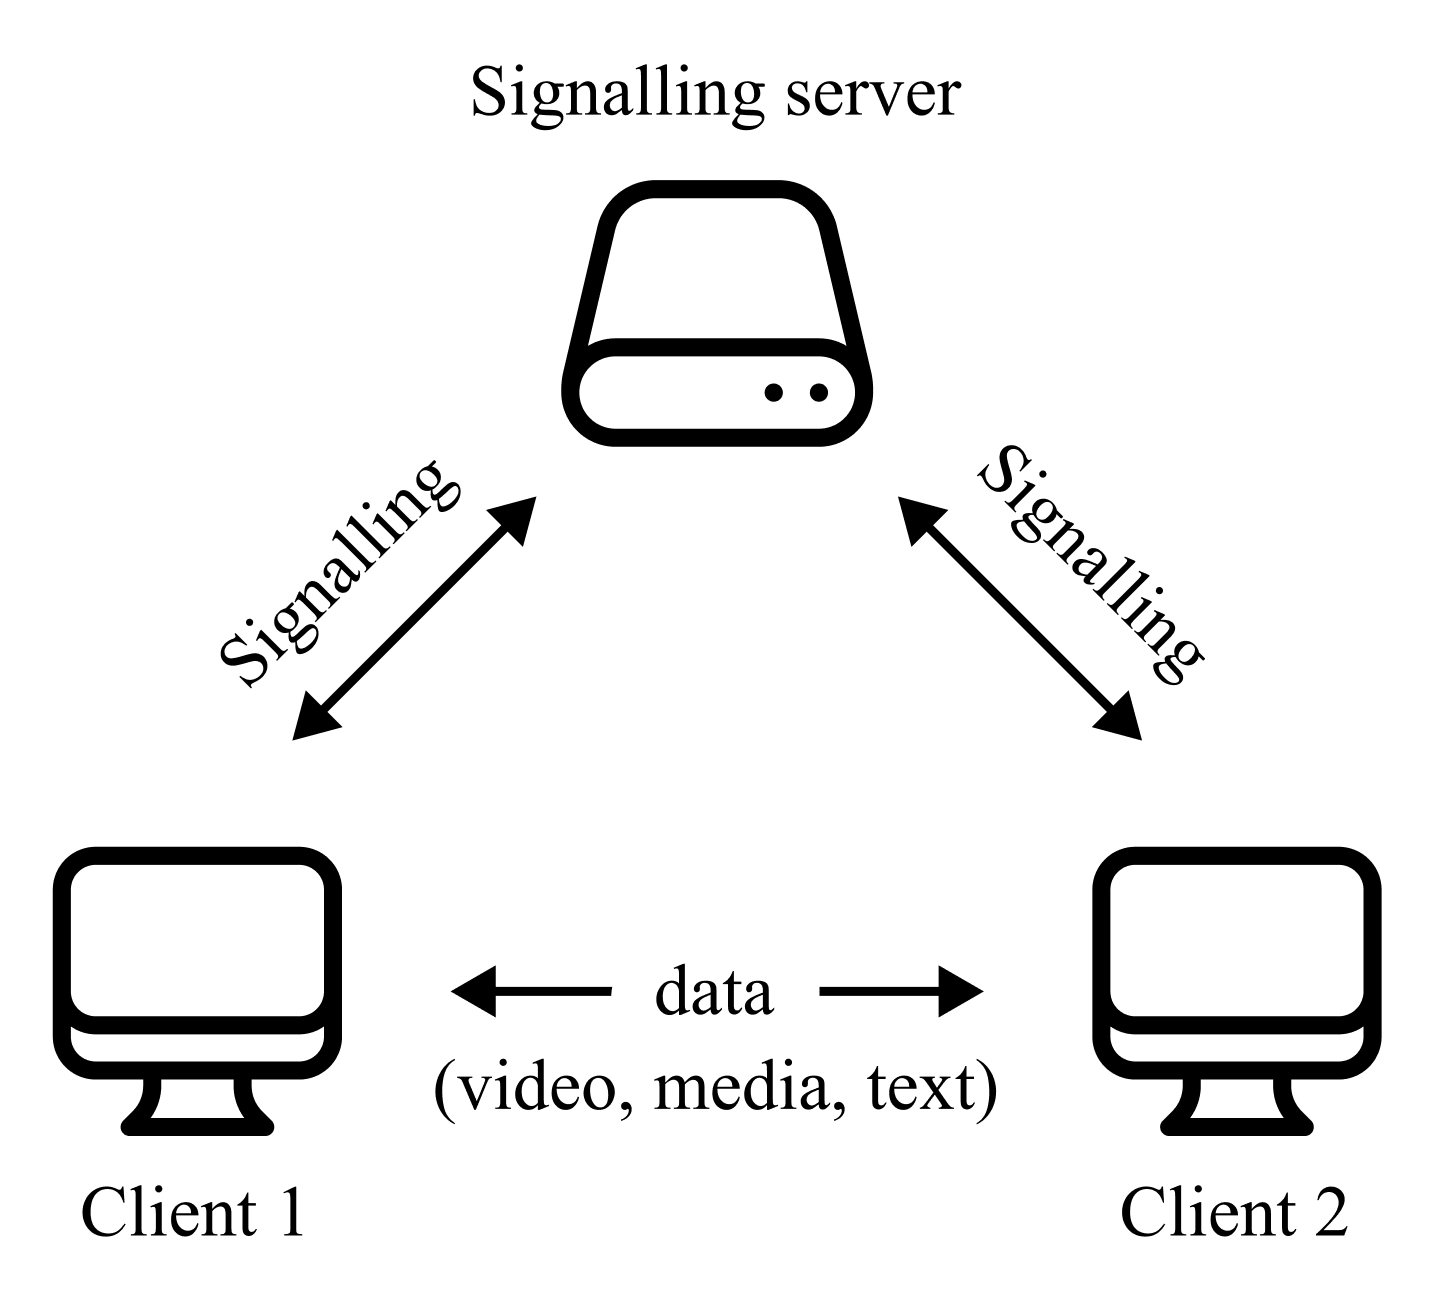
\includegraphics[width=5cm]{dissertation/images/web-rtc-diagram.png}
    \caption{WebRTC}
    \label{fig:webRTC}
\end{figure}

\section{Open Source}
\text Open source pertains to a licensing model for software that enables the public to view and modify the source code. It is developed and maintained by a community of contributors, rather than by a single entity. The objective of open source is to promote collaboration, transparency, and innovation in software development, and to give users more control and choice over their software. Notable open source projects include the Linux operating system and the Python programming language.

\section{Existing Projects}
\text The Espruino project is an ambitious attempt at bringing embedded systems programming to the masses through an easy to get started with ecosystem which takes advantage of many in house tools to provide the best experience possible for the developers. These tools aim to not change the way we develop but extend upon it through the usage of the below tools we can see this approach.

\subsection{Espruino JavaScript language}
The \href{https://www.espruino.com/Reference#top}{Espruino native language} is an extension of the standard JavaScript library introducing embedded systems specific keywords such as \textit{SetWatch} and pin manipulation through the syntax \textit{PIN.method()}. The addition of these keywords allow developers to interact and control embedded devices in a manor akin to alternatives such as Arduino or Micro Python. This extension of of the language transforms JavaScript into a capable systems programming language aimed at Espruino micro controller boards.

\subsection{Espruino IDE}
The \href{https://www.espruino.com/ide/}{Espruino IDE} provides an online platform for developers to get started working with their espruino devices without the need to set up any local environments. This web application provides many features such as device console logs and programming directly onto the device all round providing a perfect learning environment for new programmers whilst also acting as an ideal debugging environment for more experienced developers.

\begin{figure}[!ht]
    \centering
    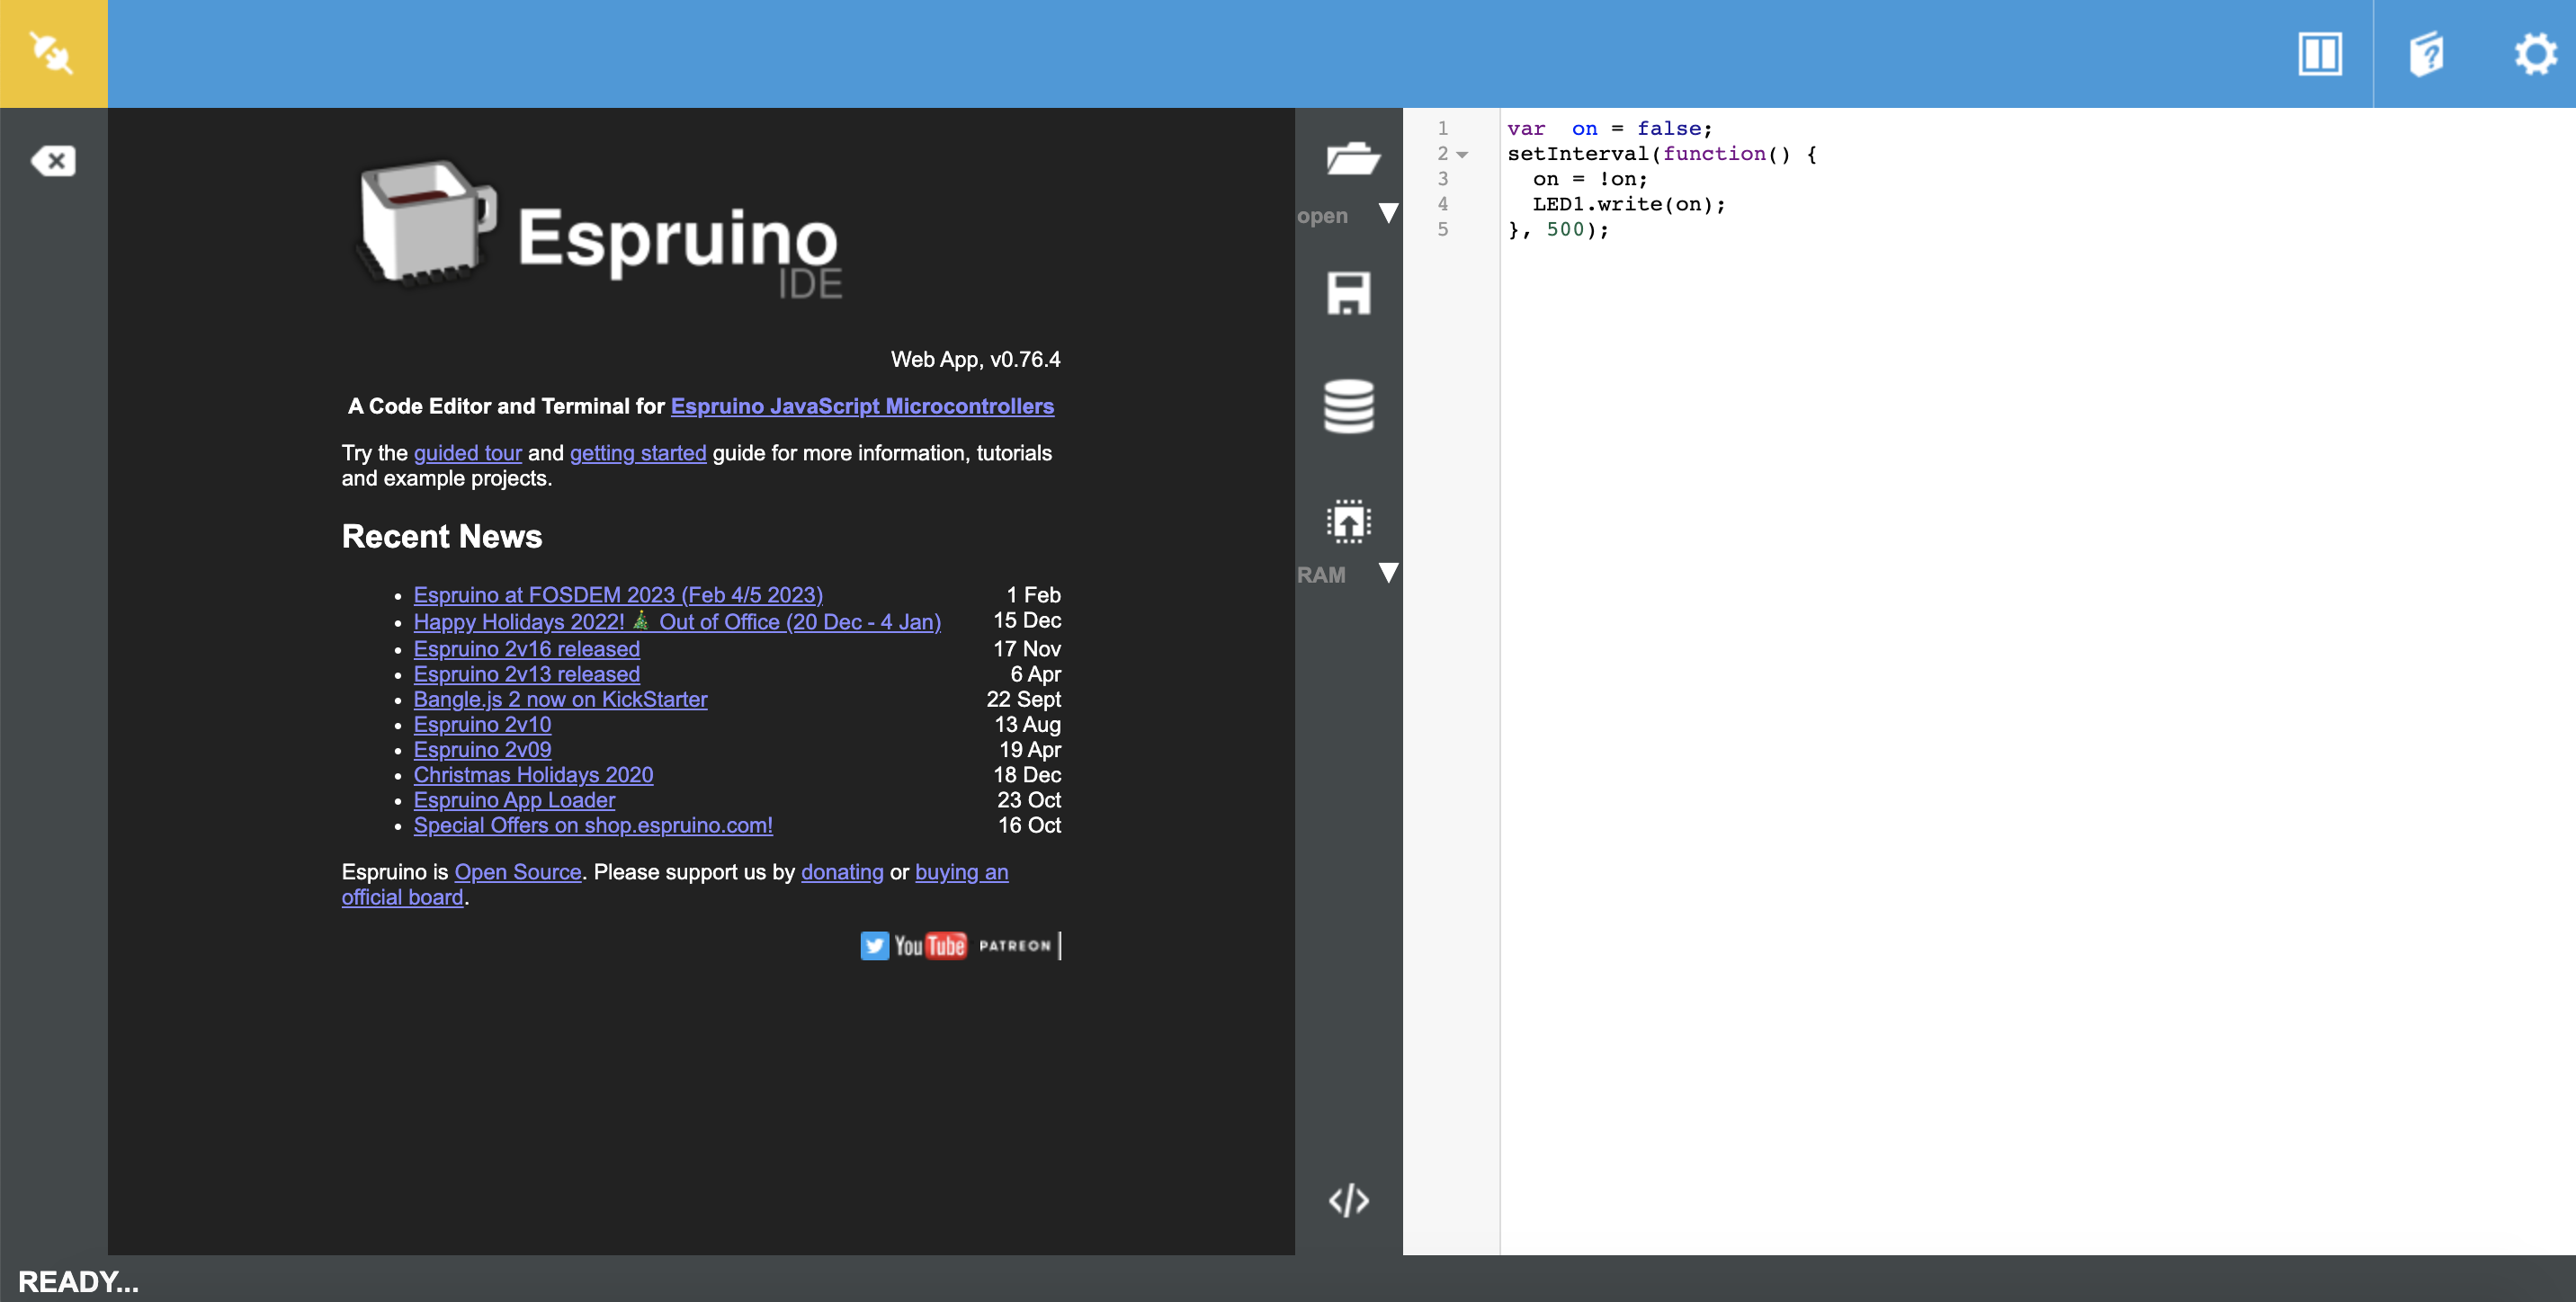
\includegraphics[width=10cm]{dissertation/images/espruino-ide.png}
    \caption{Espruino IDE}
    \label{fig:espruino-ide}
\end{figure}

%==================================================================================================================================
\chapter{Analysis/Requirements}

\text Due to the nature of this project having multiple smaller packages / applications the analysis of these mini projects were done separately. To accomplish this a MOSCOW analysis was undertaken on each project individually. Below is a compilation of the main points from these individual analysis including overlapping themes and important points from each project with the full MOSCOW requirements for each project referenced within the appendix \ref{appendix:MOSCOWAnalysis}.

\section{Problem specification}

\begin{itemize}
    \item publush information from embedded device to web page.
    \item add ability to use an espruino device almost as a javascript module.
    \item promote an environment which allows both begineers and experienced programmers to work with remote embedded devices, i.e. no limitations with straight forward syntax.
    \item remove need to write code as a string to send to device.
\end{itemize}

\section{Functional Requirements}
Short paragraph explaining the breakdown of the work items from the original specification
\subsection{Must Have}
\begin{itemize}
    \item A fully open-source ecosystem to allow for community contribution and overall clarity of how the project works at the code level.
    \item Clean and accessible syntax for the end developer to get started with including inline documentation through IDE comments.
    \item Improve the development process of Espruino device introducing a modular method of programming compared to the current almost terminal based approach.
\end{itemize}
\subsection{Should Have}
\begin{itemize}
    \item Support any style favoured style of programming including but not limited to JavaScript frameworks. A practice that will not discourage programmers at any level from jumping in to something they are already familiar or comfortable with. This will include imports through script tags as well as NPM.
    \item Refined user interface to ensure integration into existing sites is not a hassle nor an eyesore. This should be consistent across all products.
\end{itemize}
\subsection{Could Have}
\begin{itemize}
    \item Easily extendable packages including only the core functionality of the packages to allow developers to extend and implement features they desire without being held back by any limitations.
\end{itemize}
\section{Non-Functional Requirements}
\text What are non-functional requirements
\subsection{Must Have}
\begin{itemize}
    \item A well populated documentation site to explain the in's and out's of each package in depth.
    \item A hub for users to explore in depth projects built on the espruino-tools platform whilst allowing them to show off their own creations to the public.
    
\end{itemize} 
\subsection{Should Have}
\begin{itemize}
    \item 
\end{itemize} 

\section{Specification changes}
\subsection{Peer to Peer}
\text A separate package which allows users to easily integrate a connection between mobile devices and their browser to bridge the gap in espruino only being able to be used on specific devices.

\subsection{Transpiler}
\text Provide a program which can translate ... to fully allow for the code to work on any given espruino platform be that their online IDE or even directly written onto the device. Mention this came up after discussion about providing an online environment and ability for less boxed in code processing.

\subsection{NPX Tool}
\text Improve the time required to set up a development environment to allow more focus on the code and less on the logistics of how to get an environment set up.

\subsection{Online Environment}
\text Allow users to have an environment in which they can test new features without setting up a whole development environment. This can be used to test functionality or even develop whole projects.
%==================================================================================================================================
\chapter{Design}
How is this problem to be approached, without reference to specific implementation details? 

\section{Development}

Different packages/web applications required different approaches.

\subsection{Feedback Driven Development}
Fast iteration with focus on improving the features.
\begin{itemize}
    \item Forum feedback espruino forum
    
    \item User testing feedback from user study.
    \item \textit{supervisor feedback [NOT SURE IF THIS SHOULD STAY]}
\end{itemize}

\subsection{Test Driven Development}
Where possible this was implemented ensuring new package versions did not break anything.

\section{Organisations}
\subsection{Github}
\text something about open source, keeping everything together.
\subsection{NPM}
\text scoped packages, keeps everything together.
\section{NPX Tool Repositories}
\text why react, vue, typescript. Why have `--clean-install`, `--peer`
\subsection{Git Submodules}
\text Directory changes without package updates, framework specific updates can be done without package update.
\subsection{Tags}
\text `--clean-install` For experienced users `--template` allowing for further choice for the developer `--peer` allowing users without knowledge of webserver routing and ssl to also get started
\section{UI/UX Improvements}
\text modals, prototyping (Figma)
\section{Agile Methodologies}
\text choice for software architecture.
%==================================================================================================================================
\chapter{Tools / Technologies}

The section will discuss the usage of technologies throughout the project splitting them into relevant sections containing technologies used by specific areas of the project.

\section{General}

The packages discussed below are used throughout the full ecosystem and help provide the vital structure of the package development.

\subsection{Typescript}
\text Typescript offers several benefits over JavaScript when building a software package. It is a statically typed super-set of JavaScript, providing improved code quality through static typing and a better understanding of large code-bases through its type system. Typescript also offers better scalability with features like interfaces, classes, and modules, as well as better tooling support through better integration with modern development tools. Additionally, Typescript includes features that are part of upcoming versions of JavaScript, making code written in it future-proof.

\subsection{NPM}
\text Using the Node Package Management (NPM) system when developing a JavaScript application presents numerous benefits. NPM eases the management of packages, guaranteeing the right version is installed correctly. The NPM network boasts a significant community of developers and a vast collection of programs, minimizing the need for repeated efforts and making it easy to integrate new features. NPM standardizes the system for versioning packages and enables seamless distribution of programs to the community. The adoption of NPM also enables automation of processes like building, testing, and deploying packages, reducing the workload associated with managing the project.


\subsection{UNPKG}
\text The utilization of inline JavaScript imports through UNPKG provides numerous advantages. The ability to integrate small amounts of code through inline imports enables a fast and straightforward method for experimenting with various components and evaluating different solutions. Utilising both inline imports and NPM package imports simultaneously presents a versatile and efficient development process, empowering developers to select the most suitable approach for their project needs.

\subsection{Azure DevOps}
\text Azure DevOps is a unified platform for software development that consolidates various tools and services. It offers a complete solution for source control, continuous integration/testing/deployment, and project management. Azure DevOps streamlines the development process by providing features such as automated builds, continuous deployment, and team collaboration, outperforming alternative approaches that utilize individual tools like Jenkins or Jira.

\subsection{Webpack}
\text can use new javascript features and compile into older widely used, enables typescript.Other webpack benefits converts all code into es5 by choice (why es5)
Why not parcel or snowpack or another bundler

\subsection{React }
\text Why is react used for demos and online IDE vs Vue, Angular, vanilla or any other. Using a framework benefits.
comparing frameworks

\subsection{Husky }
Command runner for git hooks allows for commands such as linting and testing to be run on git hooks such as commits or push.
\begin{itemize}
    \item provides simple git hook usage
    \item Run linting / testing before a commit (package sanitising)
\end{itemize}
\subsection{Standard Version}
Utilised by husky this package brings features necessary for package development such as:
\begin{itemize}
    \item auto package versioning
    \item auto change log
\end{itemize}

\section{CLI tool }

The CLI tool takes a different approach in development to the NPM packages as there is a requirement to be run through the command line.

\subsection{NPX }
\text NPX is a command line package runner allowing for the execution of node based JavaScript packages through a specified command. This has avid usage within the javascript development scene for building starting point directories, popular examples include React's create-react-app and Vue's vue-cli to name a few.

\section{Peer }

Integrating a peer-to-peer connection without utilising a self built and hosted back-end system provided an issue.

\subsection{peerJS}
\text PeerJS provides an all-in-one solution which utilises WebRTC removing the issue of building a home made WebSocket back-end system to allow for real-time communication between devices this approach allows for developers to keep the simplicity of hosting static files without having to worry about the maintenance and cost of hosting of a back-end system.

\subsection{qrcode Package }
\begin{itemize}
    \item Allow easy device connection through camera
\end{itemize}

\section{Documentation }

\subsection{Docusaurus }
\text why this over jekyll, hugo. MDX, agolia search
\begin{itemize}
    \item components through MDX
    \item search
\end{itemize}

\section{Transpiler }

\subsection{Esprima }
\text why use existing parse/tokeniser, Mozilla standard for Javascript. Avoid re-inventing the wheel.
\subsection{EsCodeGen }
\text Why use this instead of building your own, Mozilla standard for Javascript. Avoid re-inventing the wheel.
%==================================================================================================================================
\chapter{Implementation}

\text Through the analysis of the projects specification a decision was made to separate functionality that is unrelated or can be used independently into their own packages or web applications. This approach resulted in the development of the following packages and web applications shown in figures \ref{fig:packages} and \ref{fig:webapps}.

\begin{figure}[!ht]
    
\begin{center}
\begin{tabular}{|p{2.25cm}|p{5.25cm}|p{5.25cm}|}
 \hline
 \multicolumn{3}{|c|}{Packages} \\
 \hline
 Name  & Github repo& Documentation\\
 \hline
Core & \href{https://github.com/espruino-tools/core}{espruino-tools/core}  & \href{https://documentation-xi-liard.vercel.app/docs/category/core}{docs/category/core}  \\

UART & \href{https://github.com/espruino-tools/uart}{espruino-tools/uart}  & \href{https://documentation-xi-liard.vercel.app/docs/category/uart}{docs/category/uart}  \\

Peer & \href{https://github.com/espruino-tools/peer}{espruino-tools/peer}  & \href{https://documentation-xi-liard.vercel.app/docs/category/peer}{docs/category/peer}  \\

Transpiler & \href{https://github.com/espruino-tools/transpiler}{espruino-tools/transpiler}  & \href{https://documentation-xi-liard.vercel.app/docs/category/transpiler}{docs/category/transpiler}  \\

CLI Tool &  \href{https://github.com/espruino-tools/create-espruino-app}{espruino-tools/create-espruino-app}  & \href{https://documentation-xi-liard.vercel.app/docs/category/create-espruino-app}{docs/category/create-espruino-app}  \\
 \hline
\end{tabular}
\end{center} 
    \caption{Packages}
    \label{fig:packages}
\end{figure}

\begin{figure}[!ht]
\begin{center}
\begin{tabular}{|p{2.25cm}|p{5.25cm}|p{5.25cm}|}
\hline
\multicolumn{3}{|c|}{Web Apps} \\
 \hline
 Name & Github repo & Site Link\\
 \hline
Online IDE & \href{https://github.com/espruino-tools/online-environment}{espruino-tools/online-environment} & \href{https://online-environment.vercel.app/}{online-environment.vercel.app} \\
Demo's Hub & \href{https://github.com/espruino-tools/demos}{espruino-tools/demos}  & \href{https://demos-mu.vercel.app/}{demos-mu.vercel.app} \\
Documentation & \href{https://github.com/espruino-tools/documentation}{espruino-tools/documentation} & \href{https://documentation-xi-liard.vercel.app/}{documentation-xi-liard.vercel.app} \\
 \hline
\end{tabular}
\end{center}
\caption{Web Apps}
\label{fig:webapps}
\end{figure}

Each of the packages has a unique dependency on each other, this choice of structure allows for users to get involved at any step and even develop their own solutions to improve their own custom work flow, the dependency graph is shown in figure \ref{fig:package_dep_graph}

%========================
%=
%= 
%= IMAGE LUCID SPARK FOR REWORK
%= https://lucid.app/lucidchart/3338b1b0-2b62-481b-abb9-bbf9ce7b7a7d/edit?rtempr=1&invitationId=inv_25f074ac-b765-41ec-999b-6795aa3640dc&page=0_0#
%= 
%= 
%========================

\begin{figure}[!ht]
    \centering
    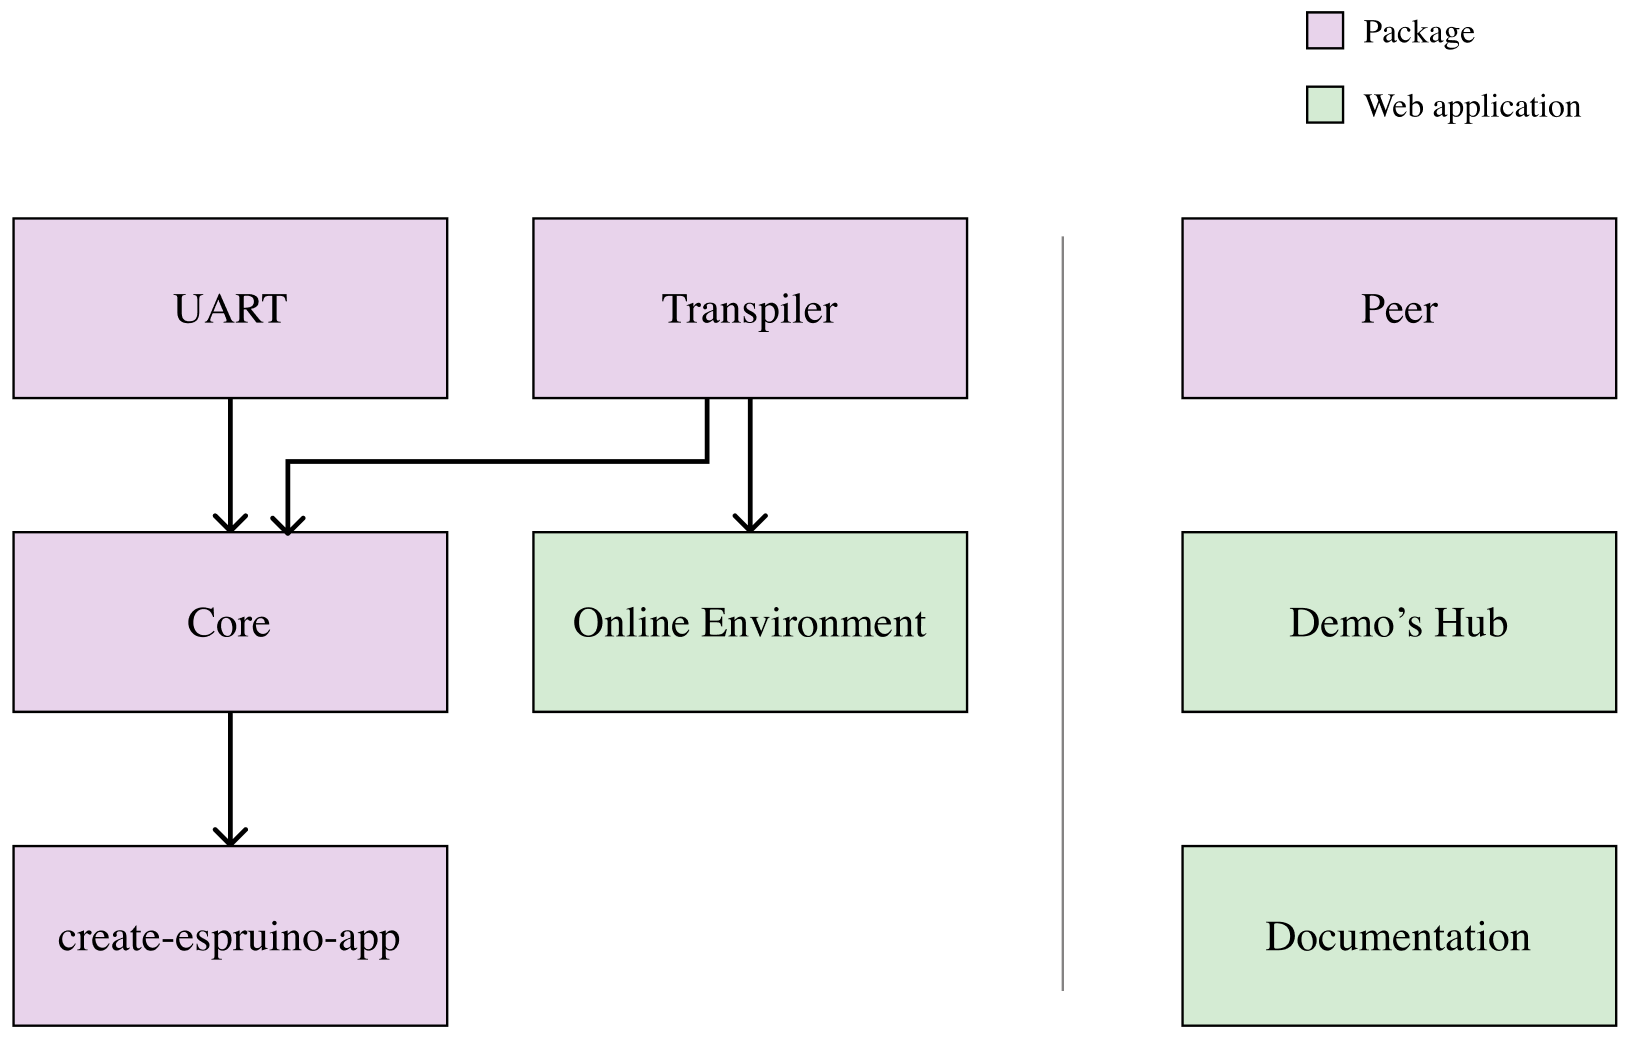
\includegraphics[width=10cm]{dissertation/images/Package_dependency_graph.jpeg}
    \caption{Dependency Graph}
    \label{fig:package_dep_graph}
\end{figure}

The packages and web applications above serve as a general view of the structure of the ecosystem the following will showcase the functionality of the packages/web applications in more detail.

\section{Packages}
Small introduction of the packages and why this approach was taken:

\begin{itemize}
    \item package approach, splitting functionality into independent parts, UNIX ideology reference.
\end{itemize}

\subsection{core}

\text What does it do.
\begin{itemize}
    \item removes need to directly send strings of code to a device.
    \item removes need for waits and provides an asynchronous model for data transfer
    \item provides a simplified approach to developing with espruino devices, \textbf{EXPLAIN WHY}.
\end{itemize}
\\
\textbf{What is impressive about it.} 
\begin{itemize}
    \item removes any confusion by incorporating everything you need into a single import based on device.
    \item allows for easy development of new devices via inheritance incorporating all basic functionality of the device (lightweight as well).
\end{itemize}
\subsection{peer}

\textbf{What does it do.}
\begin{itemize}
    \item WebRTC
    \item simplify the interaction between mobile devices and web browsers (QR Code).
\end{itemize}
\\
\textbf{What is impressive about it.}
\begin{itemize}
    \item easy to add to a site, simple configuration.
\end{itemize}
\subsection{uart}

\textbf{What does it do.}
\begin{itemize}
    \item Connection between Espruino devices and the webbrowsers
    \item improved user interaction with the package, (UI/UX)
    \item Overhaul of old package using modern javascript
\end{itemize}
\\
\textbf{What is impressive about it.}
\begin{itemize}
    \item utilises modern ECMAScript classes, allowing users to take advantage of inheritance for building their own UART implementations removing any issues with 
\end{itemize}

\subsection{create-espruino-app}

\textbf{What does it do.}
\begin{itemize}
    \item provides a simple one line command for users to get started. 
    \item provides a series of tags to customise the users development style from clean installing where no boilerplate files are provided to starting up a peer package directory.
\end{itemize}
\\
\textbf{What is impressive about it.}
\begin{itemize}
    \item Covers multiple modern development frameworks such as react and vue
\end{itemize}
\subsection{Transpiler}

\textbf{What does it do.}
\begin{itemize}
    \item Provides platform for writing core code and converting into native espruino code.
\end{itemize}
\\
\textbf{What is impressive about it.}
\begin{itemize}
    \item works as importable package and runnable CLI, allowing for full directory conversion similar to other transpiler/preprocessors such as typescript or the older coffeescript.
\end{itemize}

\section{Web Apps}

\text small paragraph about why web apps are required in this project, mention:

\begin{itemize}
    \item describe what packages do
    \item show users what the packages can do and how they can do it themselves
    \item provide an environment for users to test out functionality without committing to a project.
\end{itemize}

\subsection{online IDE}

\textbf{What does it do.}
\begin{itemize}
    \item Provides environment for online development similar to online compiler X.
\end{itemize}
\\
\textbf{What is impressive about it.}
\begin{itemize}
    \item showcases code saved on device
    \item showcases transpiled code, can be used for better understanding of the "lower level" code.
\end{itemize}

\subsection{Demo's Hub}
\textbf{What does it do.}
\begin{itemize}
    \item provides a hub for new or experienced users to browse projects built with espruino tools with easy downloading and a code viewer to see the process
\end{itemize}
\\
\textbf{What is impressive about it.}
\begin{itemize}
    \item PR based adding to site, no need for a backend Static site generation.
    \item something about config file for page population.
\end{itemize}

\section{Documentation}
\textbf{What does it do.}
\begin{itemize}
    \item place for all documentation all in one well organised place.
    \item full site searching
\end{itemize}
\\
\textbf{What is impressive about it.}
\begin{itemize}
    \item everything is built with components allowing for new pages to be built with next to no need for configuration or hassle.
\end{itemize}
\section{CI/CD}
\text The CI/CD pipeline built provides a platform the streamline the development process of the packages, this process provides the structure for how the packages are tested and prepared before deployment alongside how they are deployed leaving the developer to focus on the programming and less on the semantics of deploying an application. This is shown below in Figure \ref{fig:CICDPipeline}

\begin{figure}[!ht]
    \begin{center}
        
    
    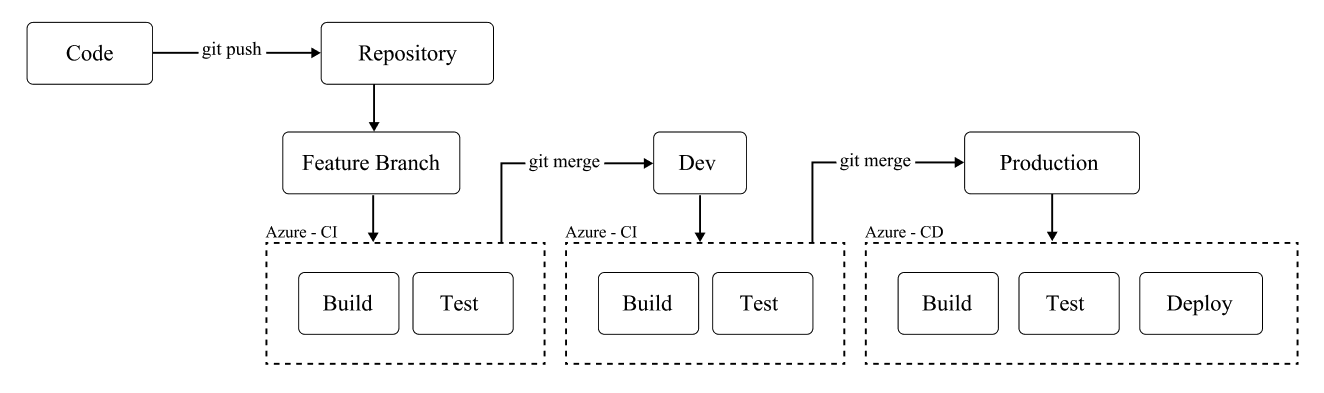
\includegraphics[width=14cm]{dissertation/images/CICD-structure.png}
    \end{center}
    \caption{CI/CD Pipeline}
    \label{fig:CICDPipeline}
\end{figure}
\\
\textbf{What does it do.}
\begin{itemize}
    \item automated testing, building, deployment.
\end{itemize}
\\
\textbf{What is impressive about it.}
\begin{itemize}
    \item automated deployment.
\end{itemize}


\section{Testing}
\text JEST, javascript testing suite. Cypress,Front end testing suite, Mocking, JSDOM. (this may only be applicable for demo site and online IDE.
\\
\textbf{What does it do.}

\\
\textbf{What is impressive about it.}



\section{Deployment}
\subsection{Packages}
\text How the packages are deployed using azure pipelines ,npm and unpkg to host package. using webpack for building minified and non minified packages (from typescript).

\begin{figure}[!ht]
    \begin{center}
    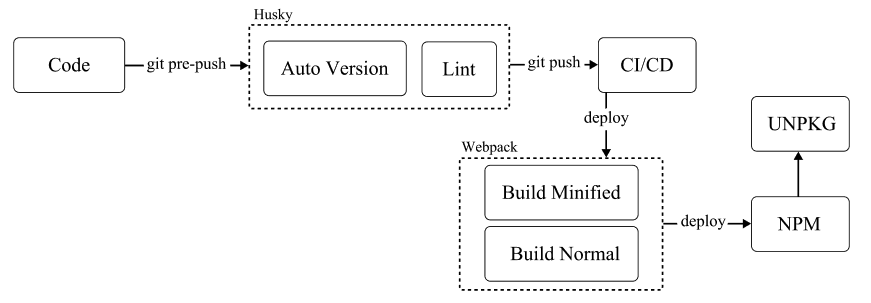
\includegraphics[width=14cm]{dissertation/images/Deployment.png}
    \end{center}
    \caption{Deployment}
    \label{fig:deployment}
\end{figure}
\\
\textbf{What does it do.}
\begin{itemize}
    \item deployed via CI/CD through npm publish, minified script is hosted automatically through UNPKG
\end{itemize}
\\
\textbf{What is impressive about it.}
\begin{itemize}
    \item automated versioning through husky.
    \item automated changelog based on commit messages.
    \item automated deployment via secondary pipeline for every package which runs on production merge after original pipeline run on development, helped via branch protection.
\end{itemize}
\subsection{Web Apps}
\text How the web apps are deployed. Vercel, what is vercel and why use it?
\\
\textbf{What does it do/what is impressive}
\begin{itemize}
    \item runs its own CI/CD ontop of mine
    \item provides deployments for development versions to test features before full production deployment.
\end{itemize}

\chapter{Evaluation} 
How good is your solution? How well did you solve the general problem, and what evidence do you have to support that?

\section{User Feedback}
\section{Core}
\subsection{Speed Comparison}
\section{Peer}
\subsection{Speed Comparison}
\section{Transpiler}

%==================================================================================================================================
\chapter{Conclusion}    
Summarise the whole project for a lazy reader who didn't read the rest (e.g. a prize-awarding committee).
\section{Summary}
\section{Reflection}
\section{Future Work}
\section{Limitation}

%==================================================================================================================================
%
% 
%==================================================================================================================================
%  APPENDICES  

\begin{appendices}
\chapter{Individual MOSCOW Analysis}


\label{appendix:MOSCOWAnalysis}

Below are the individual MOSCOW analysis of each project. These will go further into depth about the state of each individual project analysis and provide more detail surrounding the priorities.

%== CORE

\section{Core}
\subsection{Must Have}
\begin{itemize}
    \item Implement all device specific functionality into Device Objects
    \item Provide a more readable syntax for beginner users without restricting functionality
    \item Support TypeScript
    \item Be open-source
    \item Support any package import method (i.e. NPM, script tag imports)
\end{itemize}
\subsection{Should Have}
\begin{itemize}
    \item The ability to call on device functions that are already on the device.
    \item Functionality to gather device code in a readable manor, (gather functions on the device with parameters)
    \item upload code to the device.
\end{itemize}
\subsection{Could Have}
\begin{itemize}
    \item In-line documentation for package usage in IDE
\end{itemize}

%== UART

\section{UART}
\subsection{Must Have}
\begin{itemize}
    \item Improved UI/UX (cleaner modal, option to close modal)
    \item Support Typescript
    \item Be open-source
    \item Support any package import method (i.e. NPM, script tag imports)
\end{itemize}
\subsection{Should Have}
\begin{itemize}
    \item Speed Improvements (remove unused code, reduce package size, replace waits with promises)
    \item Improve device detection, current IOS detection does not work and WebBluetooth is not compatible with IOS.
    \item Use more readable javascript/typescript (original used bad code practices such as repeated code, bad variable names, global variables for everything)
\end{itemize}
\subsection{Could Have}
\begin{itemize}
    \item Call log to see what was last called on device.
    \item In-line documentation for package usage in local IDE.
\end{itemize}
\subsection{Would be nice to Have}
\begin{itemize}
    \item Options on creation for user specified maximum wiat time for device response.
\end{itemize}

%== PEER

\section{Peer}
\subsection{Must Have}
\begin{itemize}
    \item Support Typescript.
    \item Be open source.
    \item Support any package import method (i.e. NPM, script tag).
    \item Simplify setup of peerjs package to suit a standard use case without limiting the usage.

\end{itemize}
\subsection{Should Have}
\begin{itemize}
    \item Provide QR code for device connection.
    \item Support simultaneous front and back camera streaming.

\end{itemize}
\subsection{Could Have}
\begin{itemize}
    \item Provide notifications to show users connection has been initialised or closed.
    \item In-line documentation for package usage in IDE

\end{itemize}
\subsection{Would be nice to Have}
\begin{itemize}
    \item Have consistent styling with UART package.
\end{itemize}

%== TRANSPILER

\section{Transpiler}
\subsection{Must Have}
\begin{itemize}
    \item Support Typescript
    \item Be open source
    \item Support any package import method (i.e. NPM, script tag)

\end{itemize}
\subsection{Should Have}
\begin{itemize}
    \item Convert code regardless of syntax errors (for usage with newly released commands in espruino spec that arent currently supported).
    \item Support modern javascript syntax such as classes and arrow functions.
    \item Have options to transpile modules or scripts.

\end{itemize}
\subsection{Could Have}
\begin{itemize}
    \item A CLI tool to build full directories into espruino native code.
    \item In-line documentation for package usage in IDE

\end{itemize}

%== CLI TOOL

\section{CLI Tool}
\begin{itemize}
    \item 
\end{itemize}
\subsection{Must Have}
\begin{itemize}
    \item Be open source
    \item Create a working directory with the latest versions of the core package.

\end{itemize}
\subsection{Should Have}
\begin{itemize}
    \item Support multiple frameworks / coding templates such as typescript, react, vue and plain javascript.
    \item Have a template for peer setup allowing users to get started with the peer package.
    \item Error handling for incorrect command input to prevent a directory from being built on failure.

\end{itemize}
\subsection{Could Have}
\begin{itemize}
    \item Have clear progress letting the user know where the tool is in its installing progress.
\end{itemize}
\subsection{Would be nice to Have}
\begin{itemize}
    \item Support for custom templates via a github clone and set of commands to be run
\end{itemize}

%== ONLINE ENVIRONMENT

\section{Online Environment}
\subsection{Must Have}
\begin{itemize}
    \item Be open source
    \item Support live development being able to run code directly on device.
    \item Show terminal output

\end{itemize}
\subsection{Should Have}
\begin{itemize}
    \item Ability to see transpiled code.
    \item upload code from computer.
    \item save code to computer.
    \item Ability to see code on the device.

\end{itemize}
\subsection{Could Have}
\begin{itemize}
    \item Ability to save code editor code to device.
\end{itemize}
\subsection{Would be nice to Have}
\begin{itemize}
    \item A progressive web app conversion to allow for the site to be used as a local app for offline development.
\end{itemize}

%== DEMOS HUB

\section{Demos Hub}
\subsection{Must Have}
\begin{itemize}
    \item Be open source
    \item Support community uploads of demos.
    \item Show video of demo
    \item Show code from specified repository in read-only code editor.

\end{itemize}
\subsection{Should Have}
\begin{itemize}
    \item Have optionally specified links.
\end{itemize}
\subsection{Could Have}
\begin{itemize}
    \item config file to specify all information required to build the page.
\end{itemize}
\subsection{Would be nice to Have}
\begin{itemize}
    \item A page for showing users how to upload their own demos.
\end{itemize}

%== DOCUMENTATION

\section{Documentation}
\subsection{Must Have}
\begin{itemize}
    \item Be open source (Allow community edits)
    \item Accurately describe functionality of all packages
\end{itemize}
\subsection{Should Have}
\begin{itemize}
    \item Have searching functionality
    \item Provide examples of code working
\end{itemize}

\chapter{Project demos}


\label{appendix:projdemos}

\section{Core}

\begin{figure}[!ht]
    \centering
    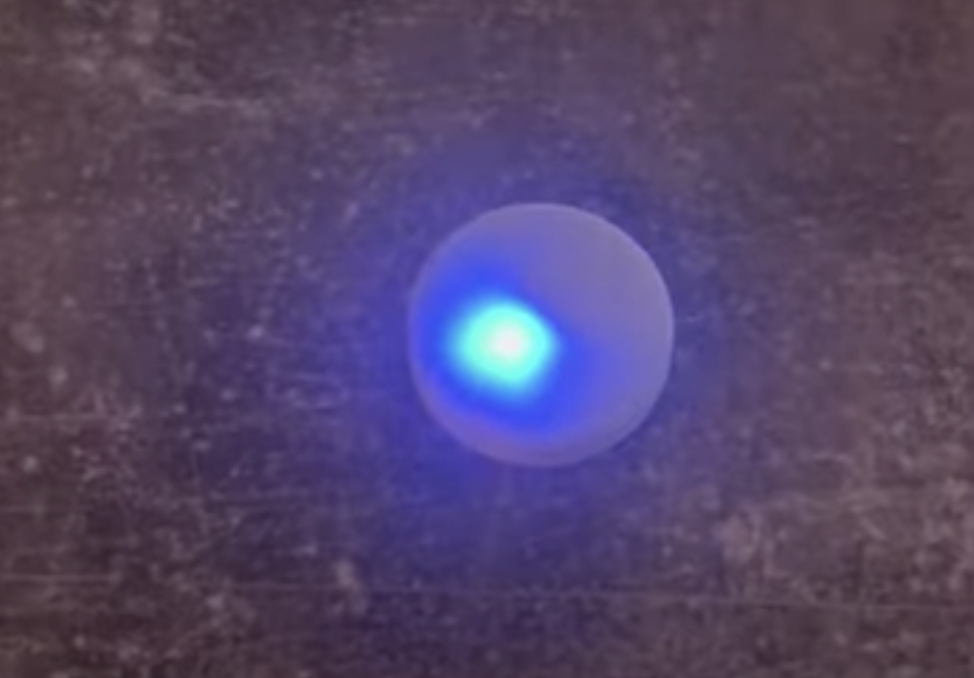
\includegraphics[width=8cm]{dissertation/images/light-sensor-demo.png}
    \caption{\href{https://demos-mu.vercel.app/demo/light-sensor}{Light Sensor Demo}}
\end{figure}



\section{Peer}
\section{Transpiler}
\section{create-espruino-app}
\end{appendices}

%==================================================================================================================================
%   BIBLIOGRAPHY   

% The bibliography style is abbrvnat
% The bibliography always appears last, after the appendices.

\bibliographystyle{abbrvnat}

\bibliography{l4proj}

\end{document}
